
\documentclass{article}
\usepackage{v-test-paper}
\newenvironment{solution}{\par\noindent\color{red!85!black}$\Rightarrow$\vspace{0em}}{}

\begin{document}

\section*{PART ONE}
\subsection*{PHYSICAL FUNDAMENTALS OF MECHANICS}
\subsubsection*{KINEMATICS}

\begin{itemize}
  \item Average vectors of velocity and acceleration of a point:
  \begin{align*}
  \intertext{where $\Delta \mathbf{r}$ is the displacement vector (an increment of a radius vector).}
  \langle \mathbf{v} \rangle &= \frac{\Delta \mathbf{r}}{\Delta t}, \quad \langle \mathbf{w} \rangle = \frac{\Delta \mathbf{v}}{\Delta t}, \tag{1.1a}
  \end{align*}
  
  \item Velocity and acceleration of a point:
  \begin{align*}
  \mathbf{v} &= \frac{d\mathbf{r}}{dt}, \quad \mathbf{w} = \frac{d\mathbf{v}}{dt}. \tag{1.1b}
  \end{align*}
  
  \item Acceleration of a point expressed in projections on the tangent and the normal to a trajectory:
    \begin{align*}
    w_t &= \frac{dv_t}{dt}, \quad w_n = \frac{v^2}{R}, \tag{1.1c}
  \intertext{where $R$ is the radius of curvature of the trajectory at the given point.}
    \end{align*}
  
  \item Distance covered by a point:
  \begin{align*}
  s &= \int v dt, \tag{1.1d}
  \intertext{where $v$ is the modulus of the velocity vector of a point.}
  \end{align*}
  
  \item Angular velocity and angular acceleration of a solid body:
  \begin{align*}
  \boldsymbol{\omega} &= \frac{d\boldsymbol{\varphi}}{dt}, \quad \boldsymbol{\beta} = \frac{d\boldsymbol{\omega}}{dt}. \tag{1.1e}
  \end{align*}
  
  \item Relation between linear and angular quantities for a rotating solid body:
  \begin{align*}
  \mathbf{v} &= \boldsymbol{\omega} r, \quad w_n = \omega^2 R, \quad \lvert w_t \rvert = \beta R, \tag{1.1f}
  \intertext{where $\mathbf{r}$ is the radius vector of the considered point relative to an arbitrary point on the rotation axis, and $R$ is the distance from the rotation axis.}
  \end{align*}
  \end{itemize}

  \pagebreak
\begin{center}
  \textsc{Problems}
\end{center}
  \begin{enumerate}[label=1.\arabic*, start=1]
    
\begin{enumerate}
    \item In a historical experiment to determine Planck's constant, a metal surface was irradiated with light of different wavelengths. The emitted photoelectron energies were measured by applying a stopping potential. The relevant data for the wavelength (\(\lambda\)) of incident light and the corresponding stopping potential (\(V_0\)) are given below:
    \begin{center}
        \begin{tabular}{ccc}
        \hline
        \(\lambda (\mu m)\) & \(V_0 (Volt)\) \\
        \hline
        0.3 & 2.0 \\
        0.4 & 1.0 \\
        0.5 & 0.4 \\
        \hline
        \end{tabular}
    \end{center}
    Given that \( c = 3 \times 10^8 m\ s^{-1} \) and \( e = 1.6 \times 10^{-19} C \), Planck's constant (in units of J s) found from such an experiment is
    \begin{tasks}(2)
        \task \( 6.0 \times 10^{-34} \)
        \task \( 6.4 \times 10^{-34} \)
        \task \( 6.6 \times 10^{-34} \)
        \task \( 6.8 \times 10^{-34} \)
    \end{tasks}
\end{enumerate}

    
\item In the arrangement of Fig. 1.9 the masses \( m_0 \), \( m_1 \), and \( m_2 \) of bodies are equal, the masses of the pulley and the threads are negligible, and there is no friction in the pulley. Find the acceleration \( w \) with which the body \( m_0 \) comes down, and the tension of the thread binding together the bodies \( m_1 \) and \( m_2 \), if the coefficient of friction between these bodies and the horizontal surface is equal to \( k \). Consider possible cases.
    \begin{center}
        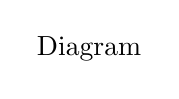
\begin{tikzpicture}
            \node at (0, 0) {Diagram};
        \end{tikzpicture}
    \end{center}

    
\begin{enumerate}
    \item A current carrying wire heats a metal rod. The wire provides a constant power (P) to the rod. The metal rod is enclosed in an insulated container. It is observed that the temperature (T) in the metal rod changes with time (t) as
    \[
    T(t) = T_0(1 + \beta t)^{\frac{1}{4}},
    \]
    where \(\beta\) is a constant with appropriate dimension while \(T_0\) is a constant with dimension of temperature. The heat capacity of the metal is;
        \begin{tasks}(2)
            \task \(\frac{4P(T(t)-T_0)^3}{\beta^4 T_0}\)
            \task \(\frac{4P(T(t)-T_0)^4}{\beta^4 T_0^5}\)
            \task \(\frac{4P(T(t)-T_0)^2}{\beta^4 T_0^3}\)
            \task \(\frac{4P(T(t)-T_0)}{\beta^4 T_0^2}\)
        \end{tasks}
\end{enumerate}

    
\item A point moves rectilinearly in one direction. Fig. 1.1 shows the distance \( s \) traversed by the point as a function of the time \( t \).
    \begin{center}
        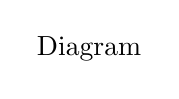
\begin{tikzpicture}
            \node at (0, 0) {Diagram}; % Replace this with the actual TikZ code for the diagram.
        \end{tikzpicture}
    \end{center}
Using the plot find:
\begin{itemize}
    \item the average velocity of the point during the time of motion;
    \item the maximum velocity;
    \item the time moment \( t_0 \) at which the instantaneous velocity is equal to the mean velocity averaged over the first \( t_0 \) seconds.
\end{itemize}

    \item A disc of mass \( m = 50 \) g slides with the zero initial velocity down an inclined plane set at an angle \( \alpha = 30^\circ \) to the horizontal; having traversed the distance \( l = 50 \) cm along the horizontal plane, the disc stops. Find the work performed by the friction forces over the whole distance, assuming the friction coefficient \( k = 0.15 \) for both inclined and horizontal planes.
    \begin{center}
        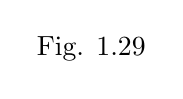
\begin{tikzpicture}
            \node at (0, 0) {Fig. 1.29};
        \end{tikzpicture}
    \end{center}\begin{solution}
    \begin{center}
        \begin{tikzpicture}
            \pic at (0, 0) {frame=3cm};
        \end{tikzpicture}
    \end{center}

    \begin{align*}
        \intertext{Let \(s\) be the distance covered by the disk along the incline, from the equation of increment of mechanical energy of the disk in the field of gravity: \(\Delta T + \Delta U - A_{fr}\)}
        0 + (-mgs\sin\alpha) &= -kmg\cos\alpha \cdot s - kmgl\\
        \intertext{or}
        s &= \dfrac{kl}{\sin\alpha - k\cos\alpha} \tag{1}
        \intertext{Hence the sought work}
        A_{fr} &= -kmg[s \cos\alpha + l]\\
        A_{fr} &= -\dfrac{klmg}{1 - k \cos\alpha} \quad \text{(using Eq. 1)}
        \intertext{On putting the values}
        A_{fr} &= -0.05 \, \text{J}
    \end{align*}
\end{solution}
    \item Two bars of masses $m_1$ and $m_2$ connected by a non-deformed light spring rest on a horizontal plane. The coefficient of friction between the bars and the surface is equal to $k$. What minimum constant force has to be applied in the horizontal direction to the bar of mass $m_1$ in order to shift the other bar?
\begin{solution}
    \begin{center}
        \begin{tikzpicture}
            \pic at (0, 0) {frame=3cm};
        \end{tikzpicture}
    \end{center}

    \begin{align*}
        \intertext{Let \(x\) be the compression in the spring when the bar \(m_2\) is about to shift. Therefore at this moment spring force on \(m_2\) is equal to the limiting friction between the bar \(m_2\) and horizontal floor. Hence}
        \kappa x &= km_2 g \quad \text{[where \(\kappa\) is the spring constant (say)]} \quad \tag{1}
        \intertext{For the block \(m_1\) from work-energy theorem:}
        A &= \Delta T = 0 \text{ for minimum force. (A here includes the work done in stretching the spring.)}
        \intertext{So,}
        Fx - \dfrac{1}{2} \kappa x^2 - km_1 g x &= 0 \quad \text{or} \quad \kappa \dfrac{x}{2} = F - km_1 g \quad \tag{2}
        \intertext{From Eqs. (1) and (2),}
        F &= kg \left(m_1 + \dfrac{m_2}{2}\right)
    \end{align*}
\end{solution}

    
\begin{enumerate}
    \item Two loudspeakers \(M\) and \(N\) are located 20 m apart and emit sound at frequencies 118 Hz and 121 Hz, respectively. A car is initially at a point \(P\), 1800 m away from the midpoint \(Q\) of the line \(MN\) and moves towards \(Q\) constantly at 60 km/hr along the perpendicular bisector of \(MN\). It crosses \(Q\) and eventually reaches a point \(R\), 1800 m away from \(Q\). Let \(v_P\), \(v_Q\) and \(v_R\) be the beat frequencies measured by a person sitting in the car at time \(t\). Let \(v(t)\) represent the beat frequency measured by a person sitting in the car at time \(t\). The speed of sound in air is 330 m s\(^{-1}\). Which of the following statement(s) is(are) true regarding the sound heard by the person?
        \begin{tasks}(1)
            \task \(v_P + v_R = 2 v_Q\)
            \task The rate of change in beat frequency is maximum when the car passes through \(Q\)
            \task The plot below represents schematically the variation of beat frequency with time (with a labeled diagram indicating points \(P\), \(Q\), and \(R\).)
            \task The plot below represents schematically the variation of beat frequency with time (with a labeled diagram indicating points \(P\), \(Q\), and \(R\).)
        \end{tasks}
\end{enumerate}
\begin{center}
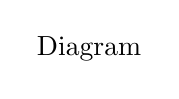
\begin{tikzpicture}
\node {Diagram};
\end{tikzpicture}
\end{center}

    
\item A spherical metal shell A of radius $R_A$ and a solid metal sphere B of radius $R_B$ ($R_B < R_A$) are kept far apart and each is given charge $`+Q'$. Now they are connected by a thin metal wire. Then
    \begin{tasks}(2)
        \task $E_{\text{inside}}^A = 0$
        \task $Q_A > Q_B$
        \task $\frac{\sigma_A}{\sigma_B} = \frac{R_B}{R_A}$
        \task $E_{\text{on surface}}^A < E_{\text{on surface}}^B$
    \end{tasks}

    
\begin{enumerate}
\item A ball is thrown from ground at an angle $\theta$ with horizontal and with an initial speed $u_0$. For the resulting projectile motion, the magnitude of average velocity of the ball up to the point when it hits the ground for the first time is $V_1$. After hitting the ground, the ball rebounds at the same angle $\theta$ but with a reduced speed of $u_0/\alpha$. Its motion continues for a long time as shown in figure. If the magnitude of average velocity of the ball for entire duration of motion is $0.8 V_1$, the value of $\alpha$ is \_\_\_\_\_\_\_.

\begin{center}
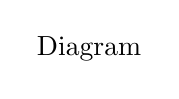
\begin{tikzpicture}
\node {Diagram};
\end{tikzpicture}
\end{center}

\end{enumerate}

    
\item A series R-C circuit is connected to AC voltage source. Consider two cases; (A) when C is without a dielectric medium and (B) when C is filled with dielectric of constant 4. The current $I_R$ through the resistor and voltage $V_C$ across the capacitor are compared in the two cases. Which of the following is/are true?
    \begin{tasks}(2)
        \task $I^A_R > I^B_R$
        \task $I^A_R < I^B_R$
        \task $V^A_C > V^B_C$
        \task $V^A_C < V^B_C$
    \end{tasks}

    
\item A cubical region of side \( a \) has its centre at the origin. It encloses three fixed point charges, \( -q \) at \( (0, -a/4, 0) \), \( +3q \) at \( (0,0,0) \) and \( -q \) at \( (0,+a/4,0) \). Choose the correct option(s).
    \begin{center}
        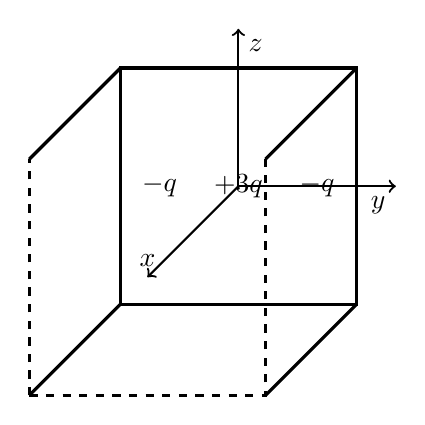
\begin{tikzpicture}
            % Drawing the cube with charges, as a simple representation
            \draw[very thick] (-1.5,-1.5,0) -- (-1.5,1.5,0) -- (1.5,1.5,0) -- (1.5,-1.5,0) -- cycle; % base
            \draw[very thick] (-1.5,-1.5,0) -- (-1.5,-1.5,3);
            \draw[very thick] (-1.5,1.5,0) -- (-1.5,1.5,3);
            \draw[very thick] (1.5,1.5,0) -- (1.5,1.5,3);
            \draw[very thick] (1.5,-1.5,0) -- (1.5,-1.5,3);

            \draw[very thick, dashed] (-1.5,-1.5,3) -- (1.5,-1.5,3) -- (1.5,1.5,3); % top
            \draw[very thick, dashed] (-1.5,-1.5,3) -- (-1.5,1.5,3);

            % Charges
            \node at (-1, 0, 0) { \( -q \) };
            \node at (0, 0, 0) { \( +3q \) };
            \node at (1, 0, 0) { \( -q \) };

            % Axes
            \draw[thick,->] (0,0,0) -- (2,0,0) node[anchor=north east] {\( y \)};
            \draw[thick,->] (0,0,0) -- (0,2,0) node[anchor=north west] {\( z \)};
            \draw[thick,->] (0,0,0) -- (0,0,3) node[anchor=south] {\( x \)};
        \end{tikzpicture}
    \end{center}
    \begin{tasks}(2)
        \task The net electric flux crossing the plane \( x = +a/2 \) is equal to the net electric flux crossing the plane \( x = -a/2 \).
        \task The net electric flux crossing the plane \( y = +a/2 \) is more than the net electric flux crossing the plane \( y = -a/2 \).
        \task The net electric flux crossing the entire region is \( \frac{q}{\varepsilon_0} \).
        \task The net electric flux crossing the plane \( z = +a/2 \) is equal to the net electric flux crossing the plane \( x = +a/2 \).
    \end{tasks}

    \item A horizontal plane with the coefficient of friction \( k \) supports two bodies: a bar and an electric motor with a battery on a block. A thread attached to the bar is wound on the shaft of the electric motor. The distance between the bar and the electric motor is equal to \( l \). When the motor is switched on, the bar, whose mass is twice as great as that of the other body, starts moving with a constant acceleration \( w \). How soon will the bodies collide?\begin{solution}
    \begin{center}
        \begin{tikzpicture}
            \pic at (0, 0) {frame=3cm};
        \end{tikzpicture}
    \end{center}
    
    \begin{align*}
        \intertext{From the Newton’s second law in projection form}
        \text{For the bar,} \quad T - 2 \ k \ m \ g &= (2m) \ w \tag{1}\\
        \text{For the motor,} \quad T - kmg &= mw' \tag{2}\\
        \intertext{Now, from the equation of kinematics in the frame of bar or motor}
        l &= \frac{1}{2} (w + w') \ t^2 \tag{3}\\
        \intertext{From Eqs. (1), (2) and (3) we get on eliminating $T$ and $w'$}
        t &= \sqrt{\frac{2l}{kg + 3w}}
    \end{align*}
\end{solution}
    


OLD MELODIES

\noindent Differentiation | \textbf{123}

\paragraph{Example 6.} The position of a particle moving along \(x\)-axis varies with time \( t \)
according as 
\[
x = t^2 - t + 1
\]
Velocity \( v_x \) and acceleration \( a_x \) of the particles are defined as
\[
v_x = \frac{dx}{dt} \quad \text{and} \quad a_x = \frac{dv_x}{dt}
\]
(i) Find velocity and acceleration at \( t = 1 \).

(ii) When is the velocity of the particle zero?

\noindent \textbf{Solution.} 
\[
v_x = \frac{dx}{dt} = \frac{d(t^2 - t + 1)}{dt} = 2t - 1
\]

\[
a_x = \frac{dv_x}{dt} = \frac{d(2t - 1)}{dt} = 2
\]

(i) At \( t = 1 \),
\[
v_x = 2 \times 1 - 1 = 1
\]
\[
a_x = 2
\]

(ii) \( v_x = 0 \)
\begin{align*}
\Rightarrow & \quad 2t - 1 = 0 \\
\Rightarrow & \quad t = \frac{1}{2} 
\end{align*}
Hence, \( v_x = 0 \) at \( t = \frac{1}{2} \)

\paragraph{Example 7.} The position of a particle moving in \( xy \)-plane varies with time \( t \)
according as 
\[
x = t + 1, \quad y = t - t^2
\]
Find \(\frac{dy}{dx}\)

\noindent \textbf{Solution.} 
\[
\frac{dy}{dx} = \frac{dy}{dt} \bigg/ \frac{dx}{dt} = \frac{d(t - t^2)}{dt} \bigg/ \frac{d(t + 1)}{dt} = \frac{(1 - 2t)}{1} = 1 - 2t
\]

\paragraph{Example 8.} The velocity \( v_x \) of a particle moving along \( x \)-axis varies with its
position \( x \) according as \( v_x = x^2 + 2x - 4 \)

Find acceleration \( a_x \) of the particle as a function of its position \( x \). Velocity \( v_x \) and acceleration \( a_x \) of the particle are defined as \( v_x = \frac{dx}{dt}, \, a_x = \frac{dv_x}{dt} \) where \( t \) denotes time

\noindent \textbf{Solution.} 
\[
a_x = \frac{dv_x}{dt}
\]
\[
\frac{dv_x}{dx} \cdot \frac{dx}{dt} = v_x \cdot \frac{dv_x}{dx}
\]
\[
a_x = (x^2 + 2x - 4) \cdot \frac{d (x^2 + 2x - 4)}{dx}
\]
\[
a_x = (x^2 + 2x - 4)(2x + 2)
\]
\[
a_x = 2 (x + 1) (x^2 + 2x - 4)
\]


    
\begin{enumerate}
    \item An optical bench has 1.5 m long scale having four equal divisions in each cm. While measuring the focal length of a convex lens, the lens is kept at 75 cm mark of the scale and the object pin is kept at 45 cm mark. The image of the object pin on the other side of the lens overlaps with image pin that is kept at 135 cm mark. In this experiment, the percentage error in the measurement of the focal length of the lens is \_\_\_\_\_\_.
\end{enumerate}

    
\begin{enumerate}
    \item A train S1, moving with a uniform velocity of 108 km/h, approaches another train S2 standing on a platform. An observer O moves with a uniform velocity of 36 km/h towards S2, as shown in figure. Both the trains are blowing whistles of same frequency 120 Hz. When O is 600 m away from S2 and distance between S1 and S2 is 800 m, the number of beats heard by O is \_\_\_\_\_\_\_\_\_. \\
    [Speed of the sound = 330 m/s]
    \begin{center}
        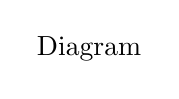
\begin{tikzpicture}
            \node {Diagram};
        \end{tikzpicture}
    \end{center}
\end{enumerate}

    \item From the photoelectric effect experiment, following observations are made. Identify which of these are correct.
    \begin{tasks}(1)
        \task The stopping potential depends only on the work function of the metal.
        \task The saturation current increases as the intensity of incident light increases.
        \task The maximum kinetic energy of a photo electron depends on the intensity of the incident light.
        \task Photoelectric effect can be explained using wave theory of light.
    \end{tasks}
    
Choose the correct answer from the options given below:
\begin{tasks}(2)
        \task B, C only
        \task A, C, D only
        \task A, B, D only
        \task B only
    \end{tasks}
     1. A stationary tuning fork is in resonance with an air column in a pipe. If the tuning fork is moved with a speed of \(2\text{ m s}^{-1}\) in front of the open end of the pipe and parallel to it, the length of the pipe should be changed for the resonance to occur with the moving tuning fork. If the speed of sound in air is \(320\text{ m s}^{-1}\), the smallest value of the percentage change required in the length of the pipe is _____.

\begin{center}
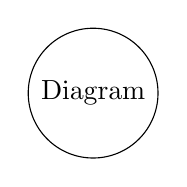
\begin{tikzpicture}
  \node [draw, shape=circle] {Diagram};
\end{tikzpicture}
\end{center}
     \item A circular disk of radius \(R\) carries surface charge density \(\sigma(r) = \sigma_0 \left(1 - \frac{r}{R}\right)\), where \(\sigma_0\) is a constant and \(r\) is the distance from the center of the disk. Electric flux through a large spherical surface that encloses the charged disk completely is \(\Phi_0\). Electric flux through another spherical surface of radius \(R-\frac{r}{4}\) and concentric with the disk is \(\Phi\). Then the ratio \(\frac{\Phi}{\Phi_0}\) is \underline{\hspace{2.5 cm}}.

 \begin{solution}
    \begin{align*}
        \intertext{Total charge on the disk, \(Q\), is obtained by integrating the surface charge density over the area of the disk,}
        Q &= \int_0^{2\pi} \int_0^R \sigma(r) r \, dr \, d\theta \\
        &= \int_0^{2\pi} \int_0^R \sigma_0 \left(1 - \frac{r}{R}\right) r \, dr \, d\theta \\
        &= \sigma_0 \int_0^{2\pi} \left(\int_0^R r - \frac{r^2}{R} \, dr\right) d\theta \\
        &= \sigma_0 \int_0^{2\pi} \left(\frac{R^2}{2} - \frac{R^3}{3R}\right) d\theta \\
        &= \sigma_0 (2\pi) \left(\frac{R^2}{2} - \frac{R^2}{3}\right) \\
        &= \sigma_0 (2\pi) \frac{R^2}{6} \\
        &= \frac{\sigma_0 \pi R^2}{3}
        \intertext{The electric flux \(\Phi_0\) through a large spherical surface enclosing the disk is given by,}
        \Phi_0 &= \frac{Q}{\varepsilon_0} \\
        &= \frac{\sigma_0 \pi R^2}{3\varepsilon_0}
        \intertext{The electric flux \(\Phi\) through a spherical surface of radius \(R-\frac{r}{4}\) is given by,}
        \Phi &= \frac{Q'}{\varepsilon_0}
        \intertext{where \(Q'\) is the charge inside the sphere of radius \(R-\frac{r}{4}\). Since the sphere is concentric with the disk, we need to find charge within radius \(R-\frac{r}{4}\),}
        Q' &= \int_0^{2\pi} \int_0^{R-\frac{r}{4}} \sigma(r) r \, dr \, d\theta \\
        &= \sigma_0 \int_0^{2\pi} \left(\int_0^{R-\frac{r}{4}} r - \frac{r^2}{R} \, dr\right) d\theta \\
        &= \sigma_0 \int_0^{2\pi} \left(\frac{(R-\frac{r}{4})^2}{2} - \frac{(R-\frac{r}{4})^3}{3R}\right) d\theta \\
        &= \sigma_0 (2\pi) \frac{(R-\frac{r}{4})^2}{6} \\
        &= \frac{\sigma_0 \pi (R-\frac{r}{4})^2}{3}
        \intertext{So, the ratio \(\frac{\Phi}{\Phi_0}\) is,}
        \frac{\Phi}{\Phi_0} &= \frac{\frac{\sigma_0 \pi (R-\frac{r}{4})^2}{3\varepsilon_0}}{\frac{\sigma_0 \pi R^2}{3\varepsilon_0}} \\
        &= \frac{(R-\frac{r}{4})^2}{R^2} \\
        &= \frac{R^2 - \frac{rR}{2} + \frac{r^2}{16}}{R^2} \\
        &= 1 - \frac{r}{2R} + \frac{r^2}{16R^2}
        \intertext{This is the required ratio of the electric fluxes.}
    \end{align*}
\end{solution}
    
    \item A horizontal circular platform of radius 0.5 m and mass 0.45 kg is free to rotate about its axis. Two massless spring toy-guns, each carrying a steel ball of mass 0.05 kg are attached to the platform at a distance 0.25 m from the centre on its either sides along its diameter (see figure). Each gun simultaneously fires the balls horizontally and perpendicular to the diameter in opposite directions. After leaving the platform, the balls have horizontal speed of 9 m\textsuperscript{-1} with respect to the ground. The rotational speed of the platform in\textsuperscript{-1} after the balls leave the platform is \underline{\hspace{2.5 cm}}.

    \begin{center}
        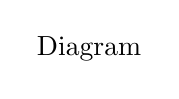
\begin{tikzpicture}
            \node {Diagram};
        \end{tikzpicture}
    \end{center}

    \item A particle of unit mass is moving along the x-axis under the influence of a force and its total energy is conserved. Four possible forms of the potential energy of the particle are given in Column I($a$ and $U_0$ are constants). Match the potential energy functions in Column I with the corresponding statement(s) in Column II.
\begin{center}
    \renewcommand{\arraystretch}{3}
    \begin{table}[h]
        \centering
        \begin{tabular}{p{0.25cm}p{5cm}|p{0.25cm}p{8cm}}
        \hline
        & Column I & & Column II \\
        \hline
        (A) & \( U_1(x) = \frac{U_0}{2} \left[ 1 - \left( \frac{x}{a} \right)^2 \right]^2 \) & (P) & The force acting on the particle is zero at \( x = a \). \\
        (B) & \( U_2(x) = \frac{U_0}{2} \left( \frac{x}{a} \right)^2 \) & (Q) & The force acting on the particle is zero at \( x = 0 \). \\
        (C) & \( U_3(x) = \frac{U_0}{2} \left( \frac{x}{a} \right)^2 \exp \left[ - \left( \frac{x}{a} \right)^2 \right] \) & (R) & The force acting on the particle is zero at \( x = -a \). \\
        (D) & \( U_4(x) = \frac{U_0}{2} \left[ \frac{x}{a} - \frac{1}{3} \left( \frac{x}{a} \right)^3 \right] \) & (S) & The particle experiences an attractive force towards \( x = 0 \) in the region \( |x| < a \). \\
         &  & (T) & The particle with total energy \( \frac{U_0}{4} \) can oscillate about the point \( x = -a \). \\
        \hline
        \end{tabular}
    \end{table}
\end{center}
\begin{solution}
    \begin{align*}
        \intertext{The force acting on the particle can be found by taking the negative derivative of the potential energy function with respect to $x$.}
        \intertext{For option (A):}
        F_1(x) &= -\dfrac{dU_1}{dx} = -\dfrac{d}{dx} \left[ \dfrac{U_0}{2} \left(1-\dfrac{x^2}{a^2}\right)^2 \right]\\
        &= -U_0 \left(\dfrac{x}{a^2}\right) \left(1-\dfrac{x^2}{a^2}\right)\\
        \intertext{The force acting on the particle is zero at \(x=0\) and \(x=\pm a\) which corresponds to option (Q) and (P)(R).}
        \intertext{For option (B):}
        F_2(x) &= -\dfrac{dU_2}{dx} = -\dfrac{d}{dx} \left[ \dfrac{U_0}{2} \left(\dfrac{x}{a}\right)^2 \right]\\
        &= -U_0 \left(\dfrac{x}{a^2}\right)\\
        \intertext{The force acting on the particle is zero at \(x=0\) which corresponds to option (Q).}
        \intertext{For option (C):}
        F_3(x) &= -\dfrac{dU_3}{dx} = -\dfrac{d}{dx} \left[ \dfrac{U_0}{2} \left(\dfrac{x}{a}\right)^2 \exp\left(-\dfrac{x^2}{a^2}\right) \right]\\
        &= -U_0 \left(\dfrac{x}{a^2}\right) \exp\left(-\dfrac{x^2}{a^2}\right) \left(1 - 2\dfrac{x^2}{a^2}\right)\\
        \intertext{The force acting on the particle is zero at \(x=0\) and \(x=\pm a/\sqrt{2}\) which corresponds to option (Q).}
        \intertext{For option (D):}
        F_4(x) &= -\dfrac{dU_4}{dx} = -\dfrac{d}{dx} \left[ \dfrac{U_0}{2} \left(\dfrac{x}{a} - \dfrac{1}{3}\left(\dfrac{x}{a}\right)^3 \right) \right]\\
        &= U_0 \left(\dfrac{1}{a} - \dfrac{x^2}{a^3}\right)\\
        \intertext{The force acting on the particle is zero at \(x=\pm a\) which corresponds to option (P) and (R). Also, in the region \(|x|<a\) the term inside the parentheses is positive, so the force acting on the particle is towards \(x=0\) which corresponds to option (S).}
    \end{align*}
\end{solution}
    \item What is the minimum acceleration with which bar \( A \) (Fig. 1.22) should be shifted horizontally to keep bodies \( 1 \) and \( 2 \) stationary relative to the bar? The masses of the bodies are equal, and the coefficient of friction between the bar and the bodies is equal to \( k \). The masses of the pulley and the threads are negligible, the friction in the pulley is absent.
    \begin{center}
        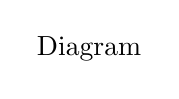
\begin{tikzpicture}
            \node at (0, 0) {Diagram};
        \end{tikzpicture}
    \end{center}
    \item Prism 1 with bar 2 of mass \( m \) placed on it gets a horizontal acceleration \( w \) directed to the left (Fig. 1.23). At what maximum value of this acceleration will the bar be still stationary relative to the prism, if the coefficient of friction between them \( k < \cot \alpha \)?
    \begin{center}
        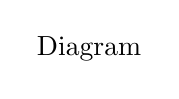
\begin{tikzpicture}
            \node at (0, 0) {Diagram};
        \end{tikzpicture}
    \end{center}
    \item Prism 1 of mass \(m_1\) and with angle \(\alpha\) (see Fig. 1.23) rests on a horizontal surface. Bar 2 of mass \(m_2\) is placed on the prism. Assuming the friction to be negligible, find the acceleration of the prism. 
    \begin{center}
        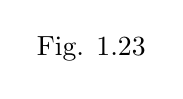
\begin{tikzpicture}
            \node at (0, 0) {Fig. 1.23};
        \end{tikzpicture}
    \end{center}\begin{solution}
    \begin{center}
        \begin{tikzpicture}
            \pic at (0, 0) {frame=3cm};
        \end{tikzpicture}
    \end{center}
    
    \begin{align*}
        \intertext{Let us draw the force diagram of each body, and on this basis we observe that the prism moves towards right (say) with an acceleration $\vec{w}_1$ and the bar 2 of mass $m_2$ moves down the plane with respect to 1, say with acceleration $\vec{w}_{21}$, then}
        \vec{w}_2 &= \vec{w}_{21} + \vec{w}_1 \quad \text{(see figure).}
        \intertext{Let us write Newton’s second law of both bodies in projection form along positive $y_2$ and $x_1$ axes as shown in the figure.}
        m_2 g \cos \alpha - N &= m_2 w_{2(y_2)} = m_2 [w_{21(y_2)} + w_{1(y_2)}] = m_2 [0 + w_1 \sin \alpha]
        \intertext{or}
        m_2 g \cos \alpha - N &= m_2 w_1 \sin \alpha \tag{1}
        \intertext{and}
        N \sin \alpha &= m_1 w_1 \tag{2}
        \intertext{Solving Eqs. (1) and (2), we get}
        w_1 &= \dfrac{m_2 g \sin \alpha \cos \alpha}{m_1 + m_2 \sin^2 \alpha} = \dfrac{g \sin \alpha \cos \alpha}{(m_1/m_2) + \sin^2 \alpha}
    \end{align*}
\end{solution}
    
\item A radius vector of a point A relative to the origin varies with time \( t \) as \( \mathbf{r} = at\mathbf{i} - bt^3\mathbf{j} \), where \( a \) and \( b \) are positive constants, and \( \mathbf{i} \) and \( \mathbf{j} \) are the unit vectors of the \( x \) and \( y \) axes. Find:
    \begin{enumerate}
        \item the equation of the point's trajectory \( y(x) \); plot this function;
        \item the time dependence of the velocity \( \mathbf{v} \) and acceleration \( \mathbf{w} \) vectors, as well as of the moduli of these quantities;
        \item the time dependence of the angle \( \alpha \) between the vectors \( \mathbf{w} \) and \( \mathbf{v} \);
        \item the mean velocity vector averaged over the first \( t \) seconds of motion, and the modulus of this vector.
    \end{enumerate}

\begin{solution}
    \begin{center}
        \begin{tikzpicture}
            \pic at (0, 0) {frame=3cm};
        \end{tikzpicture}
    \end{center}
    
    \begin{align*}
        \intertext{(a) As}
        \vec{r} &= at\hat{i} - bt^2\hat{j} \\
        \intertext{So,}
        x &= at,\ y = -bt^2 \\
        \intertext{and therefore}
        y &= \dfrac{-bx^2}{a^2}
        \intertext{which is equation of a parabola, whose graph is shown in the figure.}
        \intertext{(b) As}
        \vec{r} &= at\hat{i} - bt^2\hat{j} \\
        \intertext{So,}
        \vec{v} &= \dfrac{d\vec{r}}{dt} = a\hat{i} - 2bt\hat{j} \tag{1} \\
        v &= \sqrt{a^2 + (-2bt)^2} = \sqrt{a^2 + 4b^2t^2}
        \intertext{Differentiating Eq. (1) with respect to time, we get}
        \vec{w} &= \dfrac{d\vec{v}}{dt} = -2b\hat{j} \\
        \intertext{So,}
        |\vec{w}| &= w = 2b \\
        \intertext{(c)}
        \cos{\alpha} &= \dfrac{\vec{v} \cdot \vec{w}}{vw} = \dfrac{(a\hat{i} - 2bt\hat{j}) \cdot (-2b\hat{j})}{(\sqrt{a^2 + 4b^2 t^2}) 2b} \\
        \intertext{or}
        \cos{\alpha} &= \dfrac{2bt}{\sqrt{a^2 + 4b^2 t^2}} \\
        \intertext{So,}
        \tan{\alpha} &= \dfrac{a}{2bt}\ \text{or}\ \alpha = \tan^{-1}\left(\dfrac{a}{2bt}\right)
        \intertext{(d) The mean velocity vector}
        \left<\vec{v}\right> &= \dfrac{\int{\vec{v} dt}}{\int dt} = \dfrac{\int_0^t (a\hat{i} - 2bt\hat{j}) dt}{t} = a\hat{i} - bt\hat{j} \\
        \intertext{Hence,}
        \left<|\vec{v}|\right> &= \sqrt{a^2 + (-bt)^2} = \sqrt{a^2 + b^2 t^2}
    \end{align*}
\end{solution}

    \item A smooth light horizontal rod \(AB\) can rotate about a vertical axis passing through its end \(A\). The rod is fitted with a small sleeve of mass \(m\) attached to the end \(A\) by a weightless spring of length \(l_0\) and stiffness \(\kappa\). What work must be performed to slowly get this system going and reaching the angular velocity \(\omega\)?
\begin{solution}
    \begin{center}
        \begin{tikzpicture}
            \pic at (0, 0) {frame=3cm};
        \end{tikzpicture}
    \end{center}
    
    \begin{align*}
        \intertext{Let the deformation in the spring be $\Delta l$, when the rod $AB$ has attained the angular velocity $\omega$. From the second law of motion in projection form $F_n = mwv_n$.}
        \kappa \Delta l &= m \omega^2 \left(l_0 + \Delta l \right)  \quad \text{or} \quad \Delta l = \dfrac{m\omega^2 l_0}{\kappa - m \omega^2}
        \intertext{From the energy equation, $A_{ext}$}
        A_{ext} &= \dfrac{1}{2} mv^2 + \dfrac{1}{2} \kappa \Delta l^2\\
        &= \dfrac{1}{2} m \omega^2 \left(l_0 + \Delta l\right)^2 + \dfrac{1}{2} \kappa \Delta l^2\\
        &= \dfrac{1}{2} m \omega^2 \left( l_0 + \dfrac{m \omega^2 l_0}{\kappa - m \omega^2}\right)^2 + \dfrac{1}{2} \kappa \left(\dfrac{m \omega^2 l_0}{\kappa - m \omega^2}\right)^2
        \intertext{On solving}
        A_{ext} &= \dfrac{\kappa l_0^2 \eta \left(1 + \eta\right)}{2 \left(1 - \eta\right)^2}, \quad \text{where} \quad \eta = \dfrac{m \omega^2}{\kappa}
    \end{align*}
\end{solution}

    
\item A point moves in the plane $xy$ according to the law $x = a \sin \omega t$, $y = a(1 - \cos \omega t)$, where $a$ and $\omega$ are positive constants. Find:
    \begin{enumerate}
        \item the distance $s$ traversed by the point during the time $t$;
        \item the angle between the point's velocity and acceleration vectors.
    \end{enumerate}

    \item Two interacting particles form a closed system whose centre of inertia is at rest. Fig. 1.36 illustrates the positions of both particles at a certain moment and the trajectory of the particle of mass $m_1$. Draw the trajectory of the particle of mass $m_2$ if $m_2 = m_1/2$.
    \begin{center}
        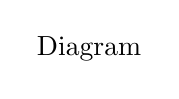
\begin{tikzpicture}
            \node at (0, 0) {Diagram};
        \end{tikzpicture}
    \end{center}\begin{solution}
    \begin{center}
        \begin{tikzpicture}
            \pic at (0, 0) {frame=3cm};
        \end{tikzpicture}
    \end{center}
    
    \begin{align*}
        \intertext{As the closed system consisting of two particles $m_1$ and $m_2$ is initially at rest, the centre of mass of the system will remain at rest. Further as $m_2 = m_1/2$, the centre of mass of the system divides the line joining $m_1$ and $m_2$ at all the moments of time in the ratio 1:2. In addition to it, the total linear momentum of the system at all the times is zero.}
        \vec{p}_1 &= -\vec{p}_2 
        \intertext{and therefore the velocities of $m_1$ and $m_2$ are also directed in opposite sense. Bearing in mind all these things, the sought trajectory is as shown in the figure.}
    \end{align*}
\end{solution}
    \item An LCR series circuit of capacitance 62.5nF and resistance of 50$\Omega$, is connected to an A.C. source of frequency 2.0 kHz. For maximum value of amplitude of current in circuit, the value of inductance is \underline{\hspace{4cm}} mH. (Take $\pi^2 = 10$)
    \item In an experiment of measuring the refractive index of a glass slab using traveling microscope in physics lab, a student measures real thickness of the glass slab as 5.25 mm and apparent thickness of the glass slab as 5.00 mm. Travelling microscope has 20 divisions in one cm on main scale and 50 divisions on vernier scale is equal to 49 divisions on main scale. The estimate uncertainly in the measurement of refractive index of the slab is $\frac{x}{10} \times 10^{-3}$, where x is \underline{\hspace{2.5cm}}.
    \item The distance between two consecutive points with phase difference of 60\(^\circ\) in a wave of frequency 500Hz is 6.0 m. The velocity with which wave is traveling is \underline{\hspace{2.5cm}} km/s.
    
\item A ball starts falling with zero initial velocity on a smooth inclined plane forming an angle $\alpha$ with the horizontal. Having fallen the distance $h$, the ball rebounds elastically off the inclined plane. At what distance from the impact point will the ball rebound for the second time?

\begin{solution}
    \begin{center}
        \begin{tikzpicture}
            \pic at (0, 0) {frame=3cm};
        \end{tikzpicture}
    \end{center}
    
    \begin{align*}
        \intertext{The ball strikes the inclined plane \( O\alpha \) at point \( O \) (origin) with velocity}
        v_0 &= \sqrt{2 gb} \tag{1}\\
        \intertext{As the ball classically rebounds, it recalls with the same velocity \( v_0 \), at the same angle \( \alpha \) from the normal on y axis (see figure). Let the ball strike the incline second time at \( P \), which is at a distance \( l \) (say) from the point \( O \), along the incline. From the equation}
        y &= v_{0_y} t + \frac{1}{2} w_y t^2\\
        0 &= v_0 \cos \alpha \tau - \frac{1}{2} g \cos \alpha \tau^2\\
        \intertext{where \( \tau \) is the time of motion of ball in air while moving from \( O \) to \( P \).}
        \intertext{As \( \tau \neq 0 \), so,}
        \tau &= \frac{2 v_0}{g} \tag{2}\\
        \intertext{Now from the equation,}
        x &= v_{0_x} t + \frac{1}{2} w_x t^2\\
        l &= v_0 \sin \alpha \tau + \frac{1}{2} g \sin \alpha \tau^2\\
        \intertext{So,}
        l &= v_0 \sin \alpha \left( \frac{2 v_0}{g} \right) + \frac{1}{2} g \sin \alpha \left( \frac{2 v_0}{g} \right)^2 = \frac{4 v_0^2 \sin \alpha}{g} \quad \text{(using Eq. 2)}\\
        \intertext{Hence the sought distance,}
        l &= \frac{4 (2 gb) \sin \alpha}{g} = 8 b \sin \alpha \quad \text{(using Eq. 1)}
    \end{align*}
\end{solution}

    \item Two small discs of masses \( m_1 \) and \( m_2 \) interconnected by a weightless spring rest on a smooth horizontal plane. The discs are set in motion with initial velocities \( v_1 \) and \( v_2 \) whose directions are mutually perpendicular and lie in a horizontal plane. Find the total energy \( \mathcal{E} \) of this system in the frame of the centre of inertia.\begin{solution}
    \begin{align*}
        \intertext{As initially \(U = \tilde{U} = 0\), so, \(\tilde{E} = \tilde{T}\). From the solution of problem 1.147(b)}
        \tilde{T} &= \dfrac{1}{2} \mu |\vec{v}_1 - \vec{v}_2|\\
        \intertext{As}
        \vec{v}_1 &\perp \vec{v}_2\\
        \intertext{Thus,}
        \tilde{T} &= \dfrac{1}{2} \dfrac{m_1 m_2}{m_1 + m_2} (v_1^2 + v_2^2)
    \end{align*}
\end{solution}
    \item A system consists of two small spheres of masses \( m_1 \) and \( m_2 \) interconnected by a weightless spring. At the moment \( t = 0 \) the spheres are set in motion with the initial velocities \( \mathbf{v_1} \) and \( \mathbf{v_2} \) after which the system starts moving in the Earth's uniform gravitational field. Neglecting the air drag, find the time dependence of the total momentum of this system in the process of motion and of the radius vector of its centre of inertia relative to the initial position of the centre.

\begin{solution}
    \begin{center}
        \begin{tikzpicture}
            \pic at (0, 0) {frame=3cm};
        \end{tikzpicture}
    \end{center}
    
    \begin{align*}
        \intertext{Velocities of masses $m_1$ and $m_2$ after $t$ seconds are, respectively,}
        \vec{v}_1' &= \vec{v}_1 + gt \tag{1.150}\\
        \vec{v}_2' &= \vec{v}_2 + gt
    \end{align*}
    
    \begin{align*}
        \intertext{Hence the final momentum of the system}
        \vec{p} &= m_1 \vec{v}_1 + m_2 \vec{v}_2 = m_1 \vec{v}_1 + m_1 \vec{v}_2 + (m_1 + m_2)gt\\
        &= \vec{p_0} + mgt \quad (\text{where, } \vec{p_0} = m_2 \vec{v}_1 + m_2 \vec{v}_2 \text{ and } m = m_1 + m_2)
    \end{align*}
    
    \begin{align*}
        \intertext{Radius vector is given by}
        \vec{r}_c &= \vec{v}_c t + \dfrac{1}{2} \vec{w}_c t^2\\
        &= \left( \dfrac{m_1 \vec{v}_1 + m_2 \vec{v}_2}{m_1 + m_2} \right)t + \dfrac{1}{2} gt^2 = \vec{v_0} t + \dfrac{1}{2} gt^2 \quad \text{where } \vec{v}_0 = \dfrac{m_1 \vec{v}_1 + m_2 \vec{v}_2}{m_1 + m_2}
    \end{align*}
    
    \begin{align*}
        \intertext{After releasing, bar 2 acquires velocity $v_2$, obtained by the energy conservation:}
        \dfrac{1}{2} m_2 v_2^2 &= \dfrac{1}{2} \kappa x^2 \quad \text{or} \quad v_2 = x \sqrt{\dfrac{\kappa}{m_2}}
    \end{align*}
    
    \begin{align*}
        \intertext{Thus, the sought velocity of C.M.}
        \vec{v}_C &= \dfrac{0 + m_2 x \sqrt{\kappa / m_2}}{m_1 + m_2} = \dfrac{x \sqrt{m_2 \kappa}}{m_1 + m_2}
    \end{align*}
\end{solution}

    
\item A balloon starts rising from the surface of the Earth. The ascension rate is constant and equal to \( v_0 \). Due to the wind the balloon gathers the horizontal velocity component \( v_x = ay \), where \( a \) is a constant and \( y \) is the height of ascent. Find how the following quantities depend on the height of ascent:
    \begin{enumerate}
        \item the horizontal drift of the balloon \( x(y) \);
        \item the total, tangential, and normal accelerations of the balloon.
    \end{enumerate}

\begin{solution}
    \begin{align*}
        \intertext{According to the problem}
        \dfrac{dy}{dt} &= v_0 \quad \text{or} \quad dy = v_0 \, dt \\
        \intertext{Integrating}
        \int_0^y dy &= v_0 \int_0^t dt \quad \text{or} \quad y = v_0 t \tag{1} \\
        \intertext{Also, we have}
        \dfrac{dx}{dt} &= ay \quad \text{or} \quad dx = ay \, dt = av_0 t \, dt \quad \text{(using Eq. 1)} \\
        \intertext{So,}
        \int_0^x dx &= av_0 \int_0^t t \, dt, \quad \text{or} \quad x = \dfrac{1}{2} av_0 t^2 = \dfrac{1}{2} a \dfrac{y^2}{v_0} \quad \text{(using Eq. 1)}
    \end{align*}
    
    \begin{align*}
        \intertext{According to the problem}
        v_y &= v_0 \quad \text{and} \quad v_x = ay \tag{2} \\
        \intertext{So,}
        v &= \sqrt{v_x^2 + v_y^2} = \sqrt{v_0^2 + ay^2} \\
        \intertext{Therefore,}
        w_t = \dfrac{dv}{dt} &= \dfrac{ay}{\sqrt{v_0^2 + ay^2}} \dfrac{dy}{dt} = \dfrac{a^2 y}{\sqrt{1 + (ay/v_0)^2}}
    \end{align*}
    
    \begin{align*}
        \intertext{Differentiating Eq. (2) with respect to time.}
        \dfrac{dy}{dt} &= w_y = 0 \quad \text{and} \quad \dfrac{dv_x}{dt} = w_x = a \dfrac{dy}{dt} = av_0 \\
        \intertext{So,}
        w = \left|w_x \right| &= av_0 \\
        \intertext{Hence,}
        w_n = \sqrt{w^2 - w_t^2} &= \sqrt{a^2 v_0^2 - \dfrac{a^2 y^2}{1 + (ay/v_0)^2}} = \dfrac{av_0}{\sqrt{1 + (ay/v_0)^2}}
    \end{align*}
\end{solution}

    \item Two bars connected by a weightless spring of stiffness \( \kappa \) and length (in the non-deformed state) \( l_0 \) rest on a horizontal plane. A constant horizontal force \( F \) starts acting on one of the bars as shown in Fig. 1.40. Find the maximum and minimum distances between the bars during the subsequent motion of the system, if the masses of the bars are:
   \begin{enumerate}
       \item equal;
       \item equal to \( m_1 \) and \( m_2 \), and the force \( F \) is applied to the bar of mass \( m_2 \).
   \end{enumerate}\begin{solution}
    \begin{center}
        \begin{tikzpicture}
            \pic at (0, 0) {frame=3cm};
        \end{tikzpicture}
    \end{center}
    
    \begin{align*}
        \intertext{Let us consider both blocks and spring as the physical system. The centre of mass of the system moves with acceleration \(a = \frac{F}{(m_{1} + m_{2})}\) towards right. Let us work in the frame of centre of mass. As this frame is a non-inertial frame (accelerated with respect to the ground) we have to apply a pseudo force \(m_{1}a\) towards left on the block \(m_{1}\) and \(m_{2}a\) towards left on the block \(m_{2}\).}\\
        \intertext{As the centre of mass is at rest in this frame, the blocks move in opposite directions and come to instantaneous rest at some instant. The elongation of the spring will be maximum or minimum at this instant. Assume that the block \(m_1\) is displaced by the distance \(x_1\) and the block \(m_2\) through a distance \(x_2\) from the initial positions.}\\
        \intertext{From the equation of increment of mechanical energy in C.M. frame}
        \Delta \widetilde{T} + \Delta U &= A_{\text{ext}}\\
        \intertext{where \(A_{\text{ext}}\) also includes the work done by the pseudo forces.}\\
        \Delta \widetilde{T} &= 0, \quad \Delta U = \frac{1}{2}k(x_{1} + x_{2})^{2} \quad \text{and}\\
        W_{\text{ext}} &= \left(F - \frac{m_{2}F}{m_{1} + m_{2}}\right)x_{2} + \frac{m_{1}F}{m_{1} + m_{2}}x_{1} = \frac{m_{1}F (x_{1} + x_{2})}{m_{1} + m_{2}}\\
        \intertext{or}
        \frac{1}{2}k(x_{1} + x_{2})^{2} &= \frac{m_{1}(x_{1} + x_{2})F}{m_{1} + m_{2}}\\
        \intertext{So,}
        x_{1} + x_{2} &= 0 \quad \text{or} \quad x_{1} + x_{2} = \frac{2m_{1}F}{k(m_{1} + m_{2})}\\
        \intertext{Hence, the maximum and minimum separations between the blocks are}\\
        l_{0} + \frac{2m_{1}F}{k (m_{1} + m_{2})} \quad \text{and} \quad l_{0}, \quad \text{respectively.}
        \intertext{Alternate:}
        \intertext{Let us link the inertial frame with horizontal floor and point the coordinate axis as shown in figure.}\\
        \intertext{At an arbitrary instant of time the separation between the blocks is \(l\) and the \(x\) coordinate of the block \(m_1\) is \(x_1\). From Newton's second law for the block \(m_1\),}
        m_{1} \frac{d^{2} x_{1}}{dt^{2}} &= k \left( l - l_{0} \right) \tag{1}\\
        \intertext{Similarly for block \(m_{2}\)}
        m_{2} \frac{d^{2} (x_{1} + l)}{dt^{2}} &= F - k \left( l - l_{0} \right) \tag{2}\\
        \intertext{Multiplying Eq. (2) by \(m_1\) and Eq. (1) by \(m_2\), and then further subtracting Eq. (1) from Eq. (2), we get}
        m_{1}m_{2} \frac{d^{2} (x + l)}{dt^{2}} - m_{1}m_{2} \frac{d^{2} x_{1}}{dt^{2}} &= m_{1}F = (m_{1} + m_{2})k (l - l_{0})\\
        \intertext{or}
        m_{1} m_{2} \frac{d^{2} l}{dt^{2}} &= m_{1}F - (m_{1} + m_{2}) k (l - l_{0}) \tag{3}\\
        \intertext{or}
        m_{1} m_{2} \frac{d^{2} (l - l_{0})}{dt^{2}} &= m_{1}F - (m_{1} + m_{2}) k (l - l_{0})\\
        \intertext{or}
        \frac{d^{2} (l - l_{0})}{dt^{2}} + \frac{k (m_{1} + m_{2})}{m_{1} m_{2}} (l - l_{0}) &= \frac{F}{m_{2}} \tag{4}\\
        \intertext{Putting \(\frac{k (m_{1} + m_{2})}{m_{1} m_{2}} = \omega^{2}\) and \(\frac{F}{m_{2}} = A\)}\\
        \intertext{and comparing with differential equation \(\frac{d^{2}x}{dt^{2}} + \omega^{2}x = A\), we get}
        l - l_{0} &= \frac{A}{\omega^{2}} + B \sin (\omega t + \delta ) \tag{5}\\
        \intertext{But at time \(t = 0\),}
        l - l_{0} &= 0 \quad \text{and} \quad \frac{d (l - l_{0})}{dt} = 0\\
        \intertext{So, \( B \omega \cos (\omega t + \delta) \vert_{t=0} = 0 \) and hence \(\delta = \frac{\pi}{2} \).}\\
        \intertext{Therefore, Eq. (5) becomes}
        l - l_{0} &= \frac{A}{\omega^{2}} + B \cos \omega t \tag{6}\\
        \intertext{But at \(t = 0\),}
        l - l_{0} &= 0, \quad \text{so,} \quad B = -\frac{A}{\omega^{2}}\\
        \intertext{Hence, Eq. (6) becomes}
        l - l_{0} &= \frac{A}{\omega^{2}} \left( 1 - \cos \omega t \right) \tag{7}\\
        \intertext{But \((l - l_{0})\) will be maximum, when \(\cos \omega t = -1\)}\\
        \intertext{Therefore, from Eq. (7)}
        l - l_{0} &= \frac{2A}{\omega^{2}} = \frac{2Fm_{1}m_{2}}{km_{2} (m_{1} + m_{2})}\\
        \intertext{or}
        l &= l_{0} + \frac{2Fm_{1}}{k(m_{1} + m_{2})}\\
        \intertext{Similarly \((l - l_{0})\) will be minimum when \(\cos \omega t = 1\)}
        \intertext{Therefore, from Eq. (7)}
        l - l_{0} &= 0 \quad \text{or} \quad l = l_{0}
    \end{align*}
\end{solution}
    \item A particle of mass \( m \) moves along the internal smooth surface of a vertical cylinder of radius \( R \). Find the force with which the particle acts on the cylinder wall if at the initial moment of time its velocity equals \( v_0 \) and forms an angle \( \alpha \) with the horizontal.\begin{solution}
    \begin{center}
        \begin{tikzpicture}
            \pic at (0, 0) {frame=3cm};
        \end{tikzpicture}
    \end{center}
    
    \begin{align*}
        \intertext{The force with which the cylinder wall acts on the particle will provide centripetal force necessary for the motion of the particle, and since there is no acceleration acting in the horizontal direction, horizontal component of the velocity will remain constant throughout the motion.}
        \text{So,} \quad v_x &= v_0 \cos \alpha \tag{1.94}
        \intertext{Using, $F_n = mw_n$, for the particle of mass $m$}
        N &= \dfrac{mv_x^2}{R} = \dfrac{mv_0^2 \cos^2 \alpha}{R}\\
        \intertext{which is the required normal force.}
    \end{align*}
\end{solution}
    \item Two identical buggies \( 1 \) and \( 2 \) with one man in each move without friction due to inertia along the parallel rails toward each other. When the buggies get opposite each other, the men exchange their places by jumping in the direction perpendicular to the motion direction. As a consequence, buggy \( 1 \) stops and buggy \( 2 \) keeps moving in the same direction, with its velocity becoming equal to \( v \). Find the initial velocities of the buggies \( v_1 \) and \( v_2 \) if the mass of each buggy (without a man) equals \( M \) and the mass of each man \( m \).
\begin{solution}
    \begin{center}
        \begin{tikzpicture}
            \pic at (0, 0) {frame=3cm};
        \end{tikzpicture}
    \end{center}
    
    \begin{align*}
        \intertext{Due to ejection of mass from a moving system (which moves due to inertia) in a direction perpendicular to it, the velocity of moving system does not change. The momentum change being adjusted by the forces on the rails. Hence in our problem velocities of buggies change only due to the entrance of the man coming from the other buggy. From conservation of linear momentum for the system (buggy 1 + man coming from buggy 2) in the direction of motion of buggy 1,}
        Mv_1 - mv_2 &= 0 \tag{1}\\
        \intertext{Similarly from conservation of linear momentum for the system (buggy 2 + man coming from buggy 1) in the direction of motion of buggy 2,}
        Mv_2 - mv_2 &= (M + m)v \tag{2}\\
        \intertext{Solving Eqs. (1) and (2), we get}
        v_1 &= \dfrac{mv}{M - m} \quad \text{and} \quad v_2 = \dfrac{Mv}{M - m}\\
        \intertext{As} 
        \vec{v_1} &\uparrow \downarrow \vec{v} \quad \text{and} \quad \vec{v_2} \uparrow \uparrow \vec{v}
        \intertext{So,}
        v_1 &= \dfrac{-mv}{M - m} \quad \text{and} \quad v_2 = \dfrac{Mv}{M - m}
    \end{align*}
\end{solution}

    
\item A point moves with deceleration along the circle of radius \( R \) so that at any moment of time its tangential and normal accelerations are equal in moduli. At the initial moment \( t = 0 \) the velocity of the point equals \( v_0 \). Find:
    \begin{center}
        
\begin{tikzpicture}
            \node at (0, 0) {diagram.png};
        \end{tikzpicture}
    \end{center}
    \begin{enumerate}
        \item the velocity of the point as a function of time and as a function of the distance covered \( s \);
        \item the total acceleration of the point as a function of velocity and the distance covered.
    \end{enumerate}

    \item Two men, each of mass $m$, stand on the edge of a stationary buggy of mass $M$. Assuming the friction to be negligible, find the velocity of the buggy after both men jump off with the same horizontal velocity $u$ relative to the buggy:
    \begin{enumerate}
        \item simultaneously;
        \item one after the other.
    \end{enumerate}
    In what case will the velocity of the buggy be greater and how many times?
\begin{solution}
    \begin{center}
        \begin{tikzpicture}
            \pic at (0, 0) {frame=3cm};
        \end{tikzpicture}
    \end{center}

    \begin{align*}
        \intertext{Let $\vec{v}_1$ be the velocity of the buggy after both men jump off simultaneously. For the closed system (two men + buggy), from the conservation of linear momentum,} 
        M\vec{v}_1 + 2m(u + \vec{v}_1) &= 0\\
        \intertext{or} 
        \vec{v}_1 &= \dfrac{-2mu}{M + 2m} \tag{1} 
        \intertext{(ii) Let $\vec{v}$ be the velocity of buggy with man, when one man jumps off the buggy. For the closed system (buggy with one man + other man) from the conservation of linear momentum:} 
        0 &= (M + m) \vec{v} + m (u + \vec{v}) \tag{2} 
        \intertext{Let $\vec{v}_2$ be the sought velocity of the buggy when the second man jumps off the buggy; then from conservation of linear momentum of the system (buggy + one man):} 
        (M + m)\vec{v} &= M\vec{v}_2 + m(u + \vec{v}_2) \tag{3} 
        \intertext{Solving Eqs. (2) and (3) we get} 
        \vec{v}_2 &= \dfrac{m(2M + 3m)u}{(M + m)(M + 2m)} \tag{4} 
        \intertext{From Eqs. (1) and (4)} 
        \dfrac{v_2}{v_1} &= 1 + \dfrac{m}{2(M + m)} &> 1 
        \intertext{Hence,} 
        v_2 &> v_1 
    \end{align*}
\end{solution}

    
\item A particle moves along an arc of a circle of radius \( R \) according to the law \( l = a \sin \omega t \), where \( l \) is the displacement from the initial position measured along the arc, and \( a \) and \( \omega \) are constants. Assuming \( R = 1.00 \, m \), \( a = 0.80 \, m \), and \( \omega = 2.00 \, rad/s \), find:
    \begin{enumerate}
        \item the magnitude of the total acceleration of the particle at the points \( l = 0 \) and \( l = \pm a \);
        \item the minimum value of the total acceleration \( w_{\text{min}} \) and the corresponding displacement \( l_m \).
    \end{enumerate}



\begin{solution}
    \begin{center}
        \begin{tikzpicture}
            \pic at (0, 0) {frame=3cm};
        \end{tikzpicture}
    \end{center}

    \begin{align*}
        \intertext{Differentiating the equation $l = a \sin \omega t$}
        \dfrac{dl}{dt} &= v = a\omega \cos \omega t\\
        w_t = \dfrac{dv}{dt} &= -a\omega^2 \sin \omega t \tag{1}
        \intertext{and}
        w_n = \dfrac{v^2}{R} &= \dfrac{a^2 \omega^2 \cos^2 \omega t}{R} \tag{2} 
        \intertext{(a) At the point $l = 0$, $\sin \omega t = 0$ and $\cos \omega t = \pm 1$ so, $\omega t = 0, \pi$, etc.}
        \intertext{Hence,}
        w = w_n &= \dfrac{a^2 \omega^2}{R} = 2.6 \, \text{m/s$^2$} \quad \text{(on substituting values)}
        \intertext{Similarly at $l = \pm a$, $\sin \omega t = \pm 1$ and $\cos \omega t = 0$, so, $w_n = 0$.}
        \intertext{Hence,}
        w = |w_t| &= a\omega^2 = 3.2 \, \text{m/s$^2$} \quad \text{(on substituting values)}
        \intertext{(b) Using $\sin \omega t = l / a$ in Eqs. (1) and (2) we get}
        w_t &= -\omega^2 l
        \intertext{and}
        w_n &= \dfrac{\omega^2}{R} \left(a^2 - l^2 \right)
        \intertext{Therefore,}
        w_l &= \sqrt{\omega^4 l^2 + \dfrac{\omega^4}{R^2} \left( a^2 - l^2\right)^2} = f(l)
        \intertext{On differentiating with respect to $l$ and putting}
        \dfrac{dw_l}{dl} &= 0
        \intertext{we get,}
        l^2 = l_m^2 &= a^2 - \dfrac{R^2}{2} = a^2 \left(1 - \dfrac{R^2}{2a^2} \right)
        \intertext{So,}
        l_m &= \pm a \sqrt{1 - \dfrac{R^2}{2a^2}} = \pm 0.37 \, \text{m} \quad \text{(on substituting values)}
        \intertext{The corresponding $w_{min}$ at $l = l_m$ is}
        w_{min} &= \sqrt{\omega^4 \left(a^2 - \dfrac{R^2}{2} \right) + \dfrac{\omega^4}{R^2} \left( \dfrac{R^2}{2}\right)^2}\\
        &= a\omega^2 \sqrt{1 - \dfrac{R^2}{2a^2} + \dfrac{R^2}{4a^2}}\\
        &= a\omega^2 \sqrt{1 - \left( \dfrac{R}{2a}\right)^2} = 2.5 \, \text{m/s$^2$} \quad \text{(on substituting values)}
    \end{align*}
\end{solution}

    
\item A point moves in the plane so that its tangential acceleration \( w_t = a \), and its normal acceleration \( w_n = bt^4 \), where \( a \) and \( b \) are positive constants, and \( t \) is time. At the moment \( t = 0 \) the point was at rest. Find how the curvature radius \( R \) of the point's trajectory and the total acceleration \( w \) depend on the distance covered \( s \).

    \item A motorboat of mass \( m \) moves along a lake with velocity \( v_0 \). At the moment \( t = 0 \) the engine of the boat is shut down. Assuming the resistance of water to be proportional to the velocity of the boat \( F = -rv \), find:
    \begin{enumerate}
        \item how long the motorboat moved with the shutdown engine;
        \item the velocity of the motorboat as a function of the distance covered with the shutdown engine, as well as the total distance covered till the complete stop;
        \item the mean velocity of the motorboat over the time interval (beginning with the moment \( t = 0 \)), during which its velocity decreases \( \eta \) times.
    \end{enumerate}\begin{solution}
    \begin{center}
        \begin{tikzpicture}
            \pic at (0, 0) {frame=3cm};
        \end{tikzpicture}
    \end{center}
    
    \begin{align*}
        \intertext{(a) From the problem $\mathbf{F} = - r \mathbf{v}$ so, $m \dfrac{d \mathbf{v}}{dt} = - r \mathbf{v}$}
        m \dfrac{dv}{dt} &= - rv \quad \text{[as $\mathbf{dv} \uparrow \downarrow \mathbf{v}$]} \\
        \dfrac{dv}{v} &= \dfrac{- r}{m} dt \\
        \intertext{On integrating}
        \ln v &= \dfrac{- r}{m} t + C \\
        \intertext{But at $t = 0$, $v = v_0$ so, $C = \ln v_0$}
        \ln \dfrac{v}{v_0} &= \dfrac{- r}{m} t \quad \text{or} \quad v = v_0 e^{(- r / m) t} \\
        \intertext{Thus, for $t \to \infty$, $v = 0$.}
        \intertext{(b) We have $m \dfrac{dv}{dt} = - rv$ so, $\dfrac{dv}{v} = \dfrac{- r}{m} ds$}
        \intertext{Integrating within the given limits to obtain $v(s)$, we get}
        \int_{v_0}^{v} dv &= \dfrac{- r}{m} \int_{0}^{s} ds \quad \text{or} \quad v = v_0 - \dfrac{rs}{m} \tag{1} \\
        \intertext{Thus for $v = 0$, $s = s_{total} = \dfrac{mv_0}{r}$}
        \intertext{(c) We have $m \dfrac{dv}{dt} = - rv$ or $\dfrac{dv}{v} = \dfrac{- r}{m} dt$}
        \begin{cases}
            \int_{0}^{v_0/ \eta} \dfrac{dv}{v} = \dfrac{- r}{m} \int_{0}^{t} dt \quad \text{or} \quad \ln \dfrac{v_0}{\eta v_0} = \dfrac{- r}{m} t \\
            \ln \dfrac{1}{\eta} = \dfrac{- r}{m} t
        \end{cases}
        \quad \text{or} \quad t = \dfrac{- m \ln \eta}{r}
        \intertext{So, $t = \dfrac{m \ln \eta}{r}$}
        \intertext{Now, average velocity over this time interval}
        <v> = \dfrac{\int v dt}{\int dt} &= \dfrac{\int_{0}^{tm \ln \eta} v_0 e^{-rt/m} dt}{tm / r \ln \eta} \\
        &= \dfrac{v_0 (\eta -1)}{\eta \ln \eta}
    \end{align*}
\end{solution}
    \item A stationary pulley carries a rope whose one end supports a ladder with a man and the other end the counterweight of mass \( M \). The man of mass \( m \) climbs up a distance \( l' \) with respect to the ladder and then stops. Neglecting the mass of the rope and the friction in the pulley axle, find the displacement \( l \) of the centre of inertia of this system.
\begin{solution}
    \begin{center}
        \begin{tikzpicture}
            \pic at (0, 0) {frame=3cm};
        \end{tikzpicture}
    \end{center}
    
    \begin{align*}
        \intertext{The displacement of the C.M. of the system, man $(m)$, ladder $(M - m)$ and the counterweight $(M)$, is described by radius vector}
        \Delta r_C &= \frac{\sum m_i \Delta r_i}{\sum m_i} = \frac{M \Delta r_M + (M - m) \Delta r_{(M-m)} + m \Delta r_m}{2M} \tag{1}\\
        \intertext{But,}
        \Delta r_m &= - \Delta r_{(M-m)}\\
        \intertext{and}
        \Delta r_m &= \Delta r_{m(M-m)} + \Delta r_{(M-m)} \tag{2}\\
        \intertext{Using Eq. (2) in Eq. (1) we get}
        \Delta r_C &= \frac{m l}{2M}
    \intertext{Alternate:}
    \intertext{Initially all the bodies of the system are at rest, and therefore the increments of linear momentum of the bodies in their motion are equal to the momentum themselves. The rope tension is the same both on the left and on the right-hand side, and consequently the momentum of the counter-balancing mass $(p_1)$ and the ladder with the man $(p_2)$ are equal at any instant of time, i.e., $p_1 = p_2$}
        M v_1 &= m v + (M - m) v_2\\
        \intertext{where $v_1,\;v,\; \text{and}\; v_2$ are the velocities of the mass, the man, and the ladder, respectively. Taking into account that $v_2 = -v_1 \; \text{and}\;v = v_2 + v'$, where $v'$ is the man's velocity relative to the ladder, we obtain}
        v_1 &= (m/2M) v'\\
        \intertext{On the other hand, the momentum of the whole system}
            p &= p_1 + p_2 = 2 p_1 \quad 2 M v_C = 2 M v_1 \tag{1}\\
        \intertext{where $V_C$ is the velocity of the centre of inertia of the system. With allowance made for Eq. (1) we get}
            V_C &= v_1 = (m/2M) v'\\
        \intertext{Finally, the sought displacement is}
        \Delta r_C &= \int V_C \, dt = (m/2M) \int v' \, dt = (m/2M) \Delta r'
    \end{align*}
\end{solution}

    
\item A wheel rotates around a stationary axis so that the rotation angle $\varphi$ varies with time as $\varphi = at^2$, where $a = 0.20 \text{ rad/s}^2$. Find the total acceleration $w$ of the point $A$ at the rim at the moment $t = 2.5 \text{ s}$ if the linear velocity of the point $A$ at this moment $v = 0.65 \text{ m/s}$.

    
\item A shell acquires the initial velocity \(v = 320 \, \text{m/s}\), having made \(n = 2.0\) turns inside the barrel whose length is equal to \(l = 2.0 \, \text{m}\). Assuming that the shell moves inside the barrel with a uniform acceleration, find the angular velocity of its axial rotation at the moment when the shell escapes the barrel.
    \begin{center}
        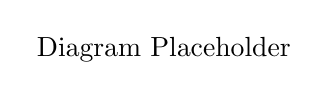
\begin{tikzpicture}
            %% Code for the actual diagram would go here. Replace the text with the corresponding TikZ commands.
            \node at (0, 0) {Diagram Placeholder};
        \end{tikzpicture}
    \end{center}

\begin{solution}
    \begin{center}
        \begin{tikzpicture}
            \pic at (0, 0) {frame=3cm};
        \end{tikzpicture}
    \end{center}
    
    \begin{align*}
        \intertext{The shell acquires a constant angular acceleration at the same time as it accelerates linearly.}
        l &= \dfrac{1}{2}wt^2 \quad \text{and} \quad 2\pi n = \dfrac{1}{2}\beta t^2\\
        \intertext{So,}
        \dfrac{w}{l} &= \dfrac{\beta}{2\pi n}\\
        \intertext{(where \( w = \) linear acceleration and \( \beta = \) angular acceleration).}
        \omega &= \sqrt{2\beta 2\pi n} = \sqrt{\dfrac{2w}{l}(2\pi n)^2}\\
        \intertext{But,}
        v^2 &= 2wl\\
        \intertext{Hence,}
        \omega &= \dfrac{2\pi nv}{l} = 2.0 \times 10^3 \text{ rad/s} \quad \text{(on substituting values)}
    \end{align*}
\end{solution}

    
\item A solid body rotates about a stationary axis according to the law $\varphi = at - bt^3$, where $a = 6.0 \text{ rad/s}^2$ and $b = 2.0 \text{ rad/s}^3$. Find:
    \begin{center}
        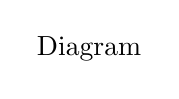
\begin{tikzpicture}
            \node at (0, 0) {Diagram}; % Replace this with the actual diagram code
        \end{tikzpicture}
    \end{center}
    \begin{enumerate}
        \item the mean values of the angular velocity and angular acceleration averaged over the time interval between $t = 0$ and the complete stop;
        \item the angular acceleration at the moment when the body stops.
    \end{enumerate}

    \item A particle of mass \( m \) moves in a certain plane \( P \) due to a force \( F \) whose magnitude is constant and whose vector rotates in that plane with a constant angular velocity \( \omega \). Assuming the particle to be stationary at the moment \( t = 0 \), find:
    \begin{center}
        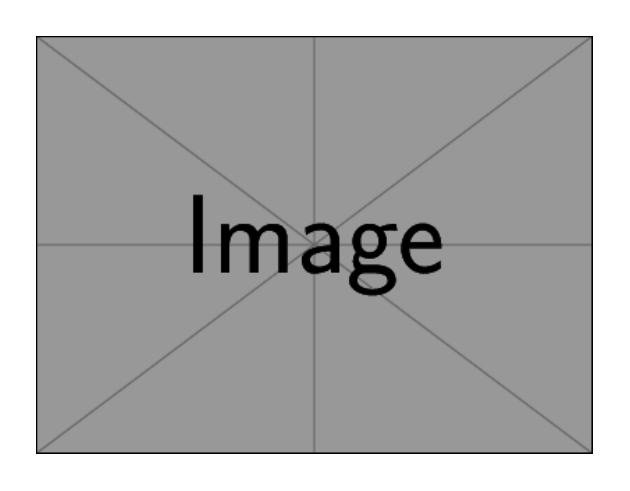
\begin{tikzpicture}
            \node at (0, 0) {\includegraphics[scale=0.5]{example-image.png}};
        \end{tikzpicture}
    \end{center}
    \begin{enumerate}
        \item its velocity as a function of time;
        \item the distance covered by the particle between two successive stops, and the mean velocity over this time.
    \end{enumerate}
    
\item A solid body rotates with deceleration about a stationary axis with an angular deceleration \(\beta \propto \sqrt{\omega}\), where \(\omega\) is its angular velocity. Find the mean angular velocity of the body averaged over the whole time of rotation if at the initial moment of time its angular velocity was equal to \(\omega_0\).

\begin{solution}
    \begin{align*}
        \intertext{In accordance with the problem, $\beta_x < 0$.}
        \text{Thus} \quad -\dfrac{d\omega}{dt} &= k \sqrt{\omega} \quad (\text{where } k \text{ is proportionality constant})\\
        \text{or} \quad -\int_{\omega_0}^{\omega} \dfrac{d\omega}{\sqrt{\omega}} &= k \int_{0}^{t} dt \quad \text{or} \quad \sqrt{\omega} = \sqrt{\omega_0} - \dfrac{kt}{2} \tag{1}\\
        \intertext{When \(\omega = 0\), total time of rotation \(t = \tau = \dfrac{2\sqrt{\omega_0}}{k}\)}
        \text{Average angular velocity} \quad <\omega> &= \dfrac{\int_{0}^{t} \omega \, dt}{\int_{0}^{t} dt} = \dfrac{\int_{0}^{2\sqrt{\omega_0}/k} \left(\omega_0 + \dfrac{k^2 t^2}{4} - kt \sqrt{\omega_0}\right) dt}{2\sqrt{\omega_0}/k}\\
        &= \dfrac{\left[ \omega_0 t + \dfrac{k^2 t^3}{12} - \dfrac{k}{2} \sqrt{\omega_0} t^2 \right]_0^{2\sqrt{\omega_0}/k}}{2\sqrt{\omega_0}/k}\\
        \intertext{Hence,}
        <\omega> &= \dfrac{\omega_0}{3}
    \end{align*}
\end{solution}

    \item A chain of length \( l \) is placed on a smooth spherical surface of radius \( R \) with one of its ends fixed at the top of the sphere. What will be the acceleration \( w \) of each element of the chain when its upper end is released? It is assumed that the length of the chain \( l < \frac{1}{2} \pi R \).
    \item A small body is placed on the top of a smooth sphere of radius $R$. Then the sphere is imparted a constant acceleration $w_0$ in the horizontal direction and the body begins sliding down. Find:
    \begin{enumerate}
        \item the velocity of the body relative to the sphere at the moment of break-off;
        \item the angle $\theta_0$ between the vertical and the radius vector drawn from the centre of the sphere to the break-off point; calculate $\theta_0$ for $w_0 = g$.
    \end{enumerate}
    
\item A rotating disc (Fig. 1.6) moves in the positive direction of the x axis. Find the equation \( y(x) \) describing the position of the instantaneous axis of rotation, if at the initial moment the axis \( C \) of the disc was located at the point \( O \) after which it moved
    \begin{enumerate}
        \item with a constant velocity \( v \), while the disc started rotating counterclockwise with a constant angular acceleration \( \beta \) (the initial angular velocity is equal to zero);
    
        \item with a constant acceleration \( w \) (and the zero initial velocity), while the disc rotates counterclockwise with a constant angular velocity \( \omega \).
    \end{enumerate}

    \item Particle 1 experiences a perfectly elastic collision with a stationary particle 2. Determine their mass ratio, if
\begin{enumerate}
    \item after a head-on collision the particles fly apart in the opposite directions with equal velocities;
    \item the particles fly apart symmetrically relative to the initial motion direction of particle 1 with the angle of divergence $\theta = 60^\circ$.
\end{enumerate}
\begin{solution}
    \begin{center}
        \begin{tikzpicture}
            \pic at (0, 0) {frame=3cm};
        \end{tikzpicture}
    \end{center}

    \begin{align*}
        \intertext{(a) Being perfectly elastic head on collision, the velocity of $i$-th particle after collision}
        \vec{v}'_i &= 2\vec{v}_C - \vec{v}_i \quad ( \text{where} \ i = 1, \ 2) \ \text{(see previous problem)}\\
        \intertext{So,}
        \vec{v}'_1 &= 2 \left( \dfrac{m_1 \vec{v}_1}{m_1 + m_2} \right) - \vec{v}_1 = \left( \dfrac{m_1 - m_2}{m_1 + m_2} \right) \vec{v}_1 \tag{1}\\
        \vec{v}'_2 &= 2 \left( \dfrac{m_1 \vec{v}_1}{m_1 + m_2} \right) \tag{2}\\
        \intertext{According to the problem}
        \vec{v}'_2 &= -\vec{v}'_1 \\
        \text{so,} \quad 2 \left( \dfrac{m_1 \vec{v}_1}{m_1 + m_2} \right) &= \left( \dfrac{m_2 - m_1}{m_1 + m_2} \right) \vec{v}_1 \ \text{which gives} \ 2m_1 = (m_2- m_1) \\
        \text{Hence,} \quad \dfrac{m_1}{m_2} &= \dfrac{1}{3}
        \intertext{(b) From conservation of linear momentum in the direction perpendicular to initial motion direction of striking particle 1 gives}
        p'_1 \sin 30^\circ &= p'_2 \sin 30^\circ \\
        \text{So,} \quad p'_1 &= p'_2 \tag{1}\\
        \intertext{From conservation of linear momentum}
        \vec{p}_1 &= \vec{p}'_1 + \vec{p}'_2, \quad \vec{p}_1 - \vec{p}'_1 = \vec{p}'_2\\
        \text{so,} \quad p^2_1 + p'^2_1 - 2p_1 p'_1 \cos 30^\circ &= p'^2_2   \tag{2}\\
        \intertext{On using Eq. (1) in Eq. (2) we get on manipulation}
        p'_1 &= \dfrac{p_1}{2 \cos 30^\circ} = \dfrac{p_1}{\sqrt{3}} \tag{3}\\
        \intertext{From conservation of kinetic energy}
        \dfrac{p^2_1}{2m_1} &= \dfrac{p'^2_1}{2m_1} + \dfrac{p'^2_2}{2m_2} \\
        \intertext{On using Eq. (1) and Eq. (3), we get on solving}
        \dfrac{m_1}{m_2} &= 2
    \end{align*}
\end{solution}

    
\item A ball of radius \( R = 10.0\ cm \) rolls without slipping down an inclined plane so that its centre moves with constant acceleration
    \begin{center}
        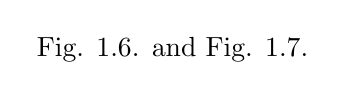
\begin{tikzpicture}
            \node at (0, 0) {Fig. 1.6. and Fig. 1.7.};
            % Diagrams should be drawn here according to the actual diagrams in the image provided
        \end{tikzpicture}
    \end{center}
    \begin{enumerate}
        \item \( w = 2.50\ cm/s^2; \quad t = 2.00\ s \) after the beginning of motion its position corresponds to that shown in Fig. 1.7. Find: the velocities of the points \( A, B, \) and \( O; \)
        \item the accelerations of these points.
    \end{enumerate}
\begin{solution}
    \begin{center}
        \begin{tikzpicture}
            \pic at (0, 0) {frame=3cm};
        \end{tikzpicture}
    \end{center}
    
    \begin{align*}
        \intertext{As the ball rolls without slipping on the rigid surface along a line so, contact point O has zero velocity, which is possible when the ball rotates in clockwise sense if its centre moves towards right and such that \(v_C = \omega R\) and \(w_C = \beta R\). As motion starts at \(t = 0\) with constant acceleration \(w\) so at time \(t\), the velocity of mass centre \(C\) becomes \(v_C = wt\) and \(\omega = \dfrac{v_C}{R} = \dfrac{wt}{R}\).}
        \intertext{(a) The contact point O becomes instantaneous centre of rotation, thus, the velocity of any arbitrary point P (say) of the ball can be obtained by the relation}
        \vec{v}_P &= \omega \times \rho_{PO} \tag{1}
        \intertext{Using Eq. (1), the pictorial diagram to find the velocities of the points A and B of the ball is shown below}
        \intertext{Hence,}
        v_A &= 2v_C = 2wt = 10 \text{ cm/s}\\
        \text{and} \quad v_B &= \sqrt{2} \; v_C = \sqrt{2} \; wt = 7.1 \text{ cm/s}
        \intertext{(b) One can write for the any arbitrary point \(P\)}
        \vec{w}_P &= \vec{w}_C + \vec{w}_{PC} = \vec{w}_C + \omega^2 \; (-\rho_{PC}) + (\beta \times \rho_{PC}) \tag{2}
        \intertext{Taking into account Eq. (2), one can easily get the acceleration of the points O, A and B on using the pictorial diagram.}
        \intertext{So,}
        w_0 &= \dfrac{w t^2}{R} = 2.5 \text{ cm/s}^2\\
        w_A &= \sqrt{4w^2 + \dfrac{w^4 t^4}{R^2}} = 2w \sqrt{1 + \left(\dfrac{w t^2}{2R} \right)^2} = 5.6 \text{ cm/s}^2\\
        \text{and} \quad w_B &= \sqrt{\left(w - \dfrac{w t^2 t^2}{R} \right)^2 + w^2} = 2.5 \text{ cm/s}^2
    \end{align*}
\end{solution}
    \item A shell flying with velocity \( v = 500 \, \text{m/s} \) bursts into three identical fragments so that the kinetic energy of the system increases \( \eta = 1.5 \) times. What maximum velocity can one of the fragments obtain?

    \item Particle 1 moving with velocity \( v = 10 \, \text{m/s} \) experienced a head-on collision with a stationary particle 2 of the same mass. As a result of the collision, the kinetic energy of the system decreased by \( \eta = 1.0\% \). Find the magnitude and direction of the velocity of particle 1 after the collision.


    
\item A solid body rotates with angular velocity $\boldsymbol{\omega} = at\mathbf{i} + bt^2\mathbf{j}$, where $a = 0.50 \, \text{rad/s}^2$, $b = 0.060 \, \text{rad/s}^3$, and $\mathbf{i}$ and $\mathbf{j}$ are the unit vectors of the $x$ and $y$ axes. Find:
    \begin{enumerate}
        \item the moduli of the angular velocity and the angular acceleration at the moment $t = 10.0 \, \text{s}$;
        \item the angle between the vectors of the angular velocity and the angular acceleration at that moment.
    \end{enumerate}

    
\item A round cone with half-angle \( \alpha = 30^\circ \) and the radius of the base \( R = 5.0 \) cm rolls uniformly and without slipping over a horizontal plane as shown in Fig. 1.8. The cone apex is hinged at the point \( O \) which is on the same level with the point \( C \), the cone base centre. The velocity of point \( C \) is \( v = 10.0 \) cm/s. Find the moduli of
\begin{center}
    
\begin{tikzpicture}
        \node at (0, 0) {diagram.png};
    \end{tikzpicture}
\end{center}
\begin{enumerate}
    \item the vector of the angular velocity of the cone and the angle it forms with the vertical;
    \item the vector of the angular acceleration of the cone.
\end{enumerate}

\begin{solution}
    \begin{center}
        \begin{tikzpicture}
            \pic at (0, 0) {frame=3cm};
        \end{tikzpicture}
    \end{center}
    
    \begin{align*}
        \intertext{(a) Let the axis of the cone ($OC$) rotate in anticlockwise sense with constant angular velocity $\omega'$ and the cone itself about its own axis ($OC$) in clockwise sense with angular velocity $\omega_0$. Then the resultant angular velocity of the cone}
        \omega &= \omega' + \omega_0\\
        \intertext{As the rolling is pure the magnitudes of the vectors $\omega'$ and $\omega_0$ can be easily found from the figure as}
        \omega' &= \dfrac{v}{R \cot \alpha} \quad \text{and} \quad \omega_0 = \dfrac{v}{R}\\
        \intertext{As $\omega \perp \omega_0$, hence}
        \omega &= \sqrt{\omega'^2 + \omega_0^2}\\
        &= \sqrt{\left(\dfrac{v}{R \cot \alpha}\right)^2 + \left(\dfrac{v}{R}\right)^2}\\
        &= \dfrac{v}{R \cos \alpha} = 2.32 \text{ rad/s}
        \intertext{(b) Vector of angular acceleration}
        \beta &= \dfrac{d \omega}{dt} = \dfrac{d (\omega' + \omega_0)}{dt} = \dfrac{d \omega_0}{dt} \quad \text{(as \(\omega'\) = constant)}\\
        \intertext{If any vector $\mathbf{a}$ (say) rotates with angular velocity $\omega$ keeping its values constant then $d\mathbf{a}/dt = \omega \times \mathbf{a}$. The vector $\omega_0$ keeping its magnitude constant rotates about the $OO'$ axis with the angular velocity $\omega'$. So $d\omega_0/dt = (\omega' \times \omega_0)$. Hence}
        \beta &= \omega' \times \omega_0 \quad \text{The magnitude of the vector $\beta$ is equal to $\beta = \omega' \omega_0$ (as $\omega' \perp \omega_0$).}\\
        \intertext{So,}
        \beta &= \dfrac{v}{R \cot \alpha} \left( \dfrac{v}{R} \right)\\
        &= \dfrac{v^2}{R^2} \tan \alpha = 2.3 \text{ rad/s}^2, \text{ on putting the values of } v, R \text{ and } \alpha
        \intertext{Alternate:}
        \intertext{Vector $\omega_0$ is turning keeping the magnitude constant. To find $d\omega_0$, let us make a vector diagram as shown in the figure. The circle shown in the figure has the radius $\omega_0$ and the tail of $\omega_0$ and of $\omega_0 + d\omega_0$ coincides at the center of the circle.}
        \intertext{Let $\omega_0$ turn by the small angle $d\phi$ in the differential time interval $dt$, so $d\phi = \omega' dt$. Thus $|d\omega_0| \approx \text{arc length} = \omega_0 d\phi = \omega_0 \omega' dt$. As $\omega_0$ is along radial line and $d\omega_0$ is along the tangent in the turning sense of $\omega_0$ so $d\omega_0 \perp \omega_0$. In vector form}
        d\omega_0 &= (\omega' \times \omega_0) dt\\
        \intertext{Hence,}
        \beta &= \dfrac{d\omega_0}{dt} = (\omega' \times \omega_0)
    \end{align*}
\end{solution}

    \item A train of mass \( m = 2000 \) tons moves in the latitude \( \varphi = 60^\circ \) North. Find:
    \begin{enumerate}
        \item the magnitude and direction of the lateral force that the train exerts on the rails if it moves along a meridian with a velocity \( v = 54 \) km per hour;
        \item in what direction and with what velocity the train should move for the resultant of the inertial forces acting on the train in the reference frame fixed to the Earth to be equal to zero.
    \end{enumerate}\begin{solution}
    \begin{center}
        \begin{tikzpicture}
            \pic at (0, 0) {frame=3cm};
        \end{tikzpicture}
    \end{center}
    
    \begin{align*}
        \intertext{(a) When the train is moving along a meridian only the Coriolis force has a lateral component and its magnitude (see the previous problem) is,}
        2m\omega v \cos \theta &= 2m \omega \sin \lambda \quad (\text{here we have put } R \dot{\theta} \rightarrow v)\\
        \intertext{So,}
        F_{\text{lateral}} &= 2 \times 2000 \times 10^3 \times \dfrac{2\pi}{86400} \times \dfrac{54000}{3600} \times \dfrac{\sqrt{3}}{2}\\
        &= 3.77 \ \text{kN} \quad (\text{we write } \lambda \text{ for the latitude})
        \intertext{(b) The resultant of the inertial forces acting on the train is,}
        \vec{F}_{\text{in}} &= -2m\omega R\dot{\theta} \cos \theta \ e_{\varphi} + (m\omega^2 R \sin \theta \cos \theta + 2m \omega R \sin \theta \cos \theta \dot{\varphi}) e_{\theta}\\
        &\quad + (m\omega^2 R \sin^2 \theta + 2m \omega R \sin^2 \theta \dot{\varphi}) e_r\\
        \intertext{This vanishes if } \dot{\theta} &= 0, \ \dot{\varphi} = -\dfrac{1}{2}\omega\\
        \intertext{Thus,}
        \vec{v} &= v_{\varphi} e_{\varphi}, \ v_{\varphi} = -\dfrac{1}{2}\omega R \sin \theta = -\dfrac{1}{2}\omega R \cos \lambda\\
        &\quad (\text{we write } \lambda \text{ for the latitude here})
        \intertext{Thus the train must move from the east to west along the 60th parallel with a speed,}
        \dfrac{1}{2}\omega R \cos \lambda &= \dfrac{1}{4} \times \dfrac{2\pi}{8.64} \times 10^{-4} \times 6.37 \times 10^6 = 115.8 \ \text{m/s} \approx 420 \ \text{km/h}
    \end{align*}
\end{solution}
  \end{enumerate}


\end{document}
